\chapter{Results}
\section{Virtual Prototyping of Cell Signals}

During the course of this thesis, numerical simulations for the microchannel have been carried out. On the one side, a simulation about the shape of a \gls{gmr}-sensor signal of cells was performed, where the magnetic momentum was conveyed through \glspl{mnp} bound to their surface. On the other side, cell aggregates have been looked at in the same manner with different angles respective to the sensor. Both simulations were then correlated to a reference dipole, with the equivalent magnetic momentum distributed in the center of mass.\\
Additionally, the flow and shear field inside the channel was simulated numerically for the channel cross-section as well as for a particle near the walls. A force equilibrium simulation was also established in a basic manner. \\
Every simulation was captured in a MATLAB class ``MRCyte'', which contains material parameters and constants for all simulations above.
\subsection{Numerical investigation of immunomagnetic label density and size on quantitative magnetoresistive sensing of single cells and cell aggregates}
In order to mimic a immunomagnetically labeled cell flowing over the sensor half bridge, the planar integral of the respective \acrfull{B} was solved analytically. Here, $\mathbf{r}_i$ specifies the distance vector of a single \gls{mnp} from the sensor plane. The magnetic flux density was converted by the \gls{gmr} to a resistive change $\mathbf{R}_{sig}$ by scaling it with the \gls{gmr}-sensitivity $S$ and subsequently into a signal voltage $\mathbf{V}_{sig}$ inside the bridge branch.(\cref{eq:magneticFluxIntegral,eq:GMR-signal,eq:voltage-signal})\\
In the numerical approach, \glspl{mnp} were randomly sampled on a sphere surface with an equivalent diameter of \SI{4}{\micro\meter} or \SI{8}{\micro\meter}. Then, the signal was computed for every \gls{mnp} during every timestep. Additionally, the \gls{mnp} distribution was rotated in every iteration to resemble a rolling motion. The computed signals were then cross-correlated to the signal of a reference flux density $\mathbf{B}_{ref}$ caused by a point-like magnetic moment located in the geometric center of the same sphere.
\begin{align}
	\mathbf{B}(t) &= \sum_{i=1}^{N} \frac{1}{A_{\mathrm{Sensor}}} \int_{-\frac{l}{2}}^{\frac{l}{2}} \int_{-\frac{w}{2}}^{\frac{w}{2}} \frac{\mu_{o}}{4 \pi}\left(\frac{3 \mathbf{r}_{i}(t)\left(\mathbf{r}_{i}(t) * \mathbf{m}_{i}\right)}{\left|\mathbf{r}_{i}(t)\right|^{5}}-\frac{\mathbf{m}_{i}}{\left|\mathbf{r}_{i}(t)\right|^{3}}\right) dx dy \label{eq:magneticFluxIntegral} \\
	\mathbf{R}_{sig}(t) &= - \mathbf{B}(t) * \frac{S}{100} * R + R \label{eq:GMR-signal}\\
	\mathbf{V}_{sig}(t) &= \frac{\mathbf{R}_{sig}(t)}{R + \mathbf{R}_{sig}(t)}*V_p - \frac{V_p}{2} \label{eq:voltage-signal}
\end{align}
By its formula, cross-correlation $R_{x y}(\tau)$ yields a displacement dependent signal through its convolution of the complex conjugated reference signal $\mathrm{V}_{ref}^{*}(t)$ with the sample signal $\mathbf{V}_{sig}(t+\tau)$.(\cref{eq:xcorr}) Therefor, only the maximal correlation of this function was considered in further analyses.
\begin{equation}
	\mathrm{max}\{R_{x y}(\tau)\}=\mathrm{max}\left\{\int_{-\infty}^{\infty} \mathrm{V}_{ref}^{*}(t) \mathbf{V}_{sig}(t+\tau) dt \right\} \label{eq:xcorr}
\end{equation}

\begin{figure}
	\centering
	\begin{minipage}[t]{.24\linewidth}
		\subfloat{
			\subfigimg[height=323pt]{a}{Ressources/Simulation/GMR}			
			\phantomsubcaption
			\label{fig:sim:intro:gmr}
		}
	\end{minipage}%
	\hfill
	\begin{minipage}[b]{.7\linewidth}
		\addtocounter{subfigure}{-1}
		\subfloat{
			\subfigimg[width=\linewidth]{b}{Ressources/Simulation/ParticleCoverage}
			\phantomsubcaption
			\label{fig:sim:intro:coverage}
		} 
		\\
		\vspace{\baselineskip}	
		\addtocounter{subfigure}{-1}
		\subfloat{
			\subfigimg[width=\linewidth]{c}{Ressources/Simulation/ParticleAngle}			
			\phantomsubcaption
			\label{fig:sim:intro:angle}
		}
	\end{minipage}%	
	\capption{Particle Coverage Simulation}{(\textbf{a}) Dimensions of the \gls{gmr} Wheatstone bridge sensor: Distance d between both variable bridges (green), width w of a \gls{gmr}-sensor, length L of a sensor. (\textbf{b}) Scheme of single cell simulation: The ideal magnetic dipole in the geometric center of a sphere (\blueCircle) causes a signal deviation from the real cell signal with magnetic moment distributed on the cell surface. (\orangeCircle) (\textbf{c}) Signal shapes of different angles of two-particle aggregates lead to differing signal shapes. }
	\label{fig:sim:intro}	
\end{figure}
\todo{Signal Similarity For Cells With Varying Bead Coverages,Cross-Correlation between single dipole with sum magentic moment and surface covered with randomly distributed magnetic particles, simulation of cell rolling velocity and forces}


\clearpage
\subsection{Single Cell Signal}
Aim of these simulations is to find a measure of how magnetic labeling of a cell affects signal shape and its subsequent analysis. A single cell with a surface coverage of \SIrange{5}{99}{\percent} of a densely packed sphere was loaded randomly with \glspl{mnp} at different sizes. Then, the previously explained rolling motion over the sensor bridge was simulated with the parameters specified in \cref{tab:params:mag_sim}. After correlation of the resulting signal voltage to the reference dipole signal (\cref{fig:sim:intro:coverage}, \blueCircle) with three randomly \gls{mnp} distributions, the dependency on the coverage was evaluated. As shown in the schematic \cref{fig:sim:intro:coverage}, an increase in signal peak amplitude but also in \gls{fwhm} at growing coverage was expected . 

\begin{table}
	\centering
\begin{tabularx}{\linewidth}{cccc}
	\toprule[1pt]
	\rule[-1ex]{0pt}{2.5ex} Parameter & Unit & Value & Explanation \\	
	\midrule
	\rule[-1ex]{0pt}{2.5ex} w & \si{\meter} & \num{2.0e-6} & GMR width \\
	\rule[-1ex]{0pt}{2.5ex} l & \si{\meter} & \num{30.0e-6} & GMR length \\
	\rule[-1ex]{0pt}{2.5ex} d & \si{\meter} & \num{14.0e-6} & Distance between two sensors \\
	\rule[-1ex]{0pt}{2.5ex} $R$ & $\mathrm{\Omega}$ & 250 & GMR Resistance\\
	\rule[-1ex]{0pt}{2.5ex} $V_p$ & \si{\milli\volt} & 100 & Supply voltage\\
	\rule[-1ex]{0pt}{2.5ex} t$_{free\ layer}$ & \si{\meter} & \num{7.0e-9} & Thickness of free layer\\
	\rule[-1ex]{0pt}{2.5ex} $\mathbf{M}$ & \si{\ampere\per\meter} & \num{2.0e4} & Volume Magnetization\\
	\rule[-1ex]{0pt}{2.5ex} $V_{noise,rms}$ & \si{\volt} & \num{2.5e-6} & Artifical noise\\
	\rule[-1ex]{0pt}{2.5ex} Sim. Space & \si{\meter} & [\num{-25e-6},\num{25e-6}] & Interval around sensor center \\	
	\bottomrule[1.2pt]
\end{tabularx}
\capption{Magnetic Simulation Parameters}{Constants used inside the framework for the simulation of the magnetic field inside the \gls{gmr} Wheatstone half bridge. The volume magnetization was adapted according to the simulated particle size.}
\label{tab:params:mag_sim}
\end{table}

The expected behavior matches the data analysis (\cref{fig:sim:coverage}). Each two analyzed sphere diameters \SIlist{4;8}{\micro\meter} with \gls{mnp} sizes ranging from \SI{20}{\nano\meter} to \SI{2}{\micro\meter}, show a great \gls{sem} at low coverage. This very probably is subjected to the momenta of single particles which play a greater individual role and hence influence the signal shape significantly because the overall dipole momentum in the sensor loses homogeneity. \\
Another observable effect is related to the \gls{mnp} size. Absolute correlation differs from \SI{20}{\nano\meter} to the ten and hundered fold diameter significantly. This can be related to the magnetic momentum per \gls{mnp} as it is dependent on the volume - thus $r^3$. However, for bigger magnetic particles this does not hold true because the composition changes from pure magnetite to a polymer shell with embedded oxide core at around \SI{150}{\nano\meter}. Nevertheless, larger particles carry also greater magnetic momentum which brings also the aforementioned influence of single \glspl{mnp} into consideration for that effect. \\ 
Also, the densely packed sphere surface can evidently carry more smaller than larger \glspl{mnp}. This ranges from \num{641600} \gls{mnp} at \SI{20}{\nano\meter} to \num{81} at \SI{2}{\micro\meter} for a sphere radius of \SI{4}{\micro\meter} and limits the maximum achievable momentum. \\
In reality, a maximum immunomagnetic label density depends not on the densely packed sphere but rather on the present antigens, and association or dissociation constants. Therefore, a complete saturation coverage is not achievable under physiological conditions. This leads to the fact that any possible momentum by deposition of \SIlist{20;50}{\nano\meter} on a cell surface cannot be resolved from noise by this sensing setup.

\begin{figure}
	\centering
	\subfloat{	
		\subfigimg[height=150pt]{a}{Ressources/Simulation/Small2um}	
		\phantomsubcaption
		\label{fig:sim:coverage:small2um}
	} \hfill
	\addtocounter{subfigure}{-1}
	\subfloat{
		\subfigimg[height=150pt]{b}{Ressources/Simulation/Big2um}
		\phantomsubcaption
		\label{fig:sim:coverage:big2um}	
	} \\
	\vspace{\baselineskip}	
	\addtocounter{subfigure}{-1}
	\subfloat{	
		\subfigimg[height=150pt]{c}{Ressources/Simulation/Small4um}	
		\phantomsubcaption
		\label{fig:sim:coverage:small4um}
	}\hfill
	\addtocounter{subfigure}{-1}
	\subfloat{
		\subfigimg[height=150pt]{d}{Ressources/Simulation/Big4um}
		\phantomsubcaption
		\label{fig:sim:coverage:big4um}
	}
\capption{Coverage Dependent Signal Correlation}{\gls{mnp} coverage of a sphere with \SI{4}{\micro\meter} (\textbf{a}, \textbf{b}) and \SI{8}{\micro\meter}  diameter  (\textbf{c}, \textbf{d}) covered by magnetic particles ranging from \SIrange{20}{2000}{\nano\meter}. A cross-correlation increase which is inversely proportional to the \gls{mnp} size can be observed.}
\label{fig:sim:coverage}
\end{figure}


Also, it can be seen that the correlation approaches a maximum obtainable value for every \gls{mnp} size. Referenced for both simulated sphere diameters in (\cref{fig:sim:CorrDiff:abs}), a inverse proportionality between correlation and \gls{mnp} diameter is visible. The trend in respective maxima can be related to differences the magnetic momentum amplitude and coverage inhomogeneity. \\ 
Inter-sphere compared, maximum correlation shows also a significant decrease in for higher \gls{mnp} sizes as the particle diameter itself increases. The relative error between both sizes - as computed in \cref{eq:sim:relCorrDiff} -  is depicted in \cref{fig:sim:CorrDiff:rel}. Assuming a dependency on the available particle surface and subsequently the fraction which can be occupied by \glspl{mnp}, a quadratic fit seems appropriate.(\cref{eq:sim:quadFit}) The fit could indicate that a reference dipole cannot be discriminated from a cell at small \gls{mnp} diameters while the correlation error becomes nearly constant at great \glspl{mnp}.

\begin{align}
	\text{Relative\ Correlation\ Difference} &= 1- \frac{\max\{\text{Cross-Correlation}(d=\SI{4}{\micro\meter})\}}{\max\{\text{Cross-Correlation}(d = \SI{8}{\micro\meter})\}} \label{eq:sim:relCorrDiff}\\
	\text{Relative\ Correlation\ Difference} &= \num{-0,38532} \, {d_{MNP}}^2 + \num{3,34574} \, d_{MNP} - \num{8,49629} \label{eq:sim:quadFit}
\end{align}



\begin{figure}
		\centering
	\subfloat{
		\subfigimg[height=150pt]{a}{Ressources/Simulation/CrossCorr-Maximal}
		\phantomsubcaption
		\label{fig:sim:CorrDiff:abs}	
	} \hfill
	\addtocounter{subfigure}{-1}
	\subfloat{
		\subfigimg[height=150pt]{b}{Ressources/Simulation/CrossCorr-Error}	
		\phantomsubcaption
		\label{fig:sim:CorrDiff:rel}
	}
\capption{Maximal Cross-Correlation Differences}{(\textbf{a}) Mean coverage at \SI{99}{\percent} for \SI{4}{\micro\meter}  and \SI{8} {\micro\meter} spheres. A negative dependency on the \gls{mnp} size can be explained by the ratio of magnetic momentum per unit surface and its homogeneous distribution across the whole surface.\\ (\textbf{b}) Relative correlation error between \SI{4}{\micro\meter}  and \SI{8} {\micro\meter} spheres with a quadratic fit. The quadratic behavior could be related to the relative surface area which can occupied by magnetic momentum. (Adj. $R^2$ = \num{0.99209})}
\label{fig:sim:CorrDiff}
\end{figure}
\subsection{Cell Aggregates}
In another simulation, two \SI{200}{\nano\meter}-\gls{mnp}-covered spheres were attached to each other in differing angles and simulated flowing over the sensor. Signal similarity to a magnetic dipole in the center of a single reference sphere was computed by cross-correlation. As can be observed in \cref{fig:sim:aggregates}, correlation is identical to a single sphere at low coverages when the magnetic momentum is high enough to form a uniform magnetic field. At occupancies greater than \SI{50}{\percent}, the two attached cells have to be considered as individual dipoles in superposition and thus show a signal that carries small peaks in the center. This is shown schematically in \cref{fig:sim:intro:angle}. In term, this causes a high signal deviation from the reference and thus a low degree of correlation.
\begin{figure}
	\centering
	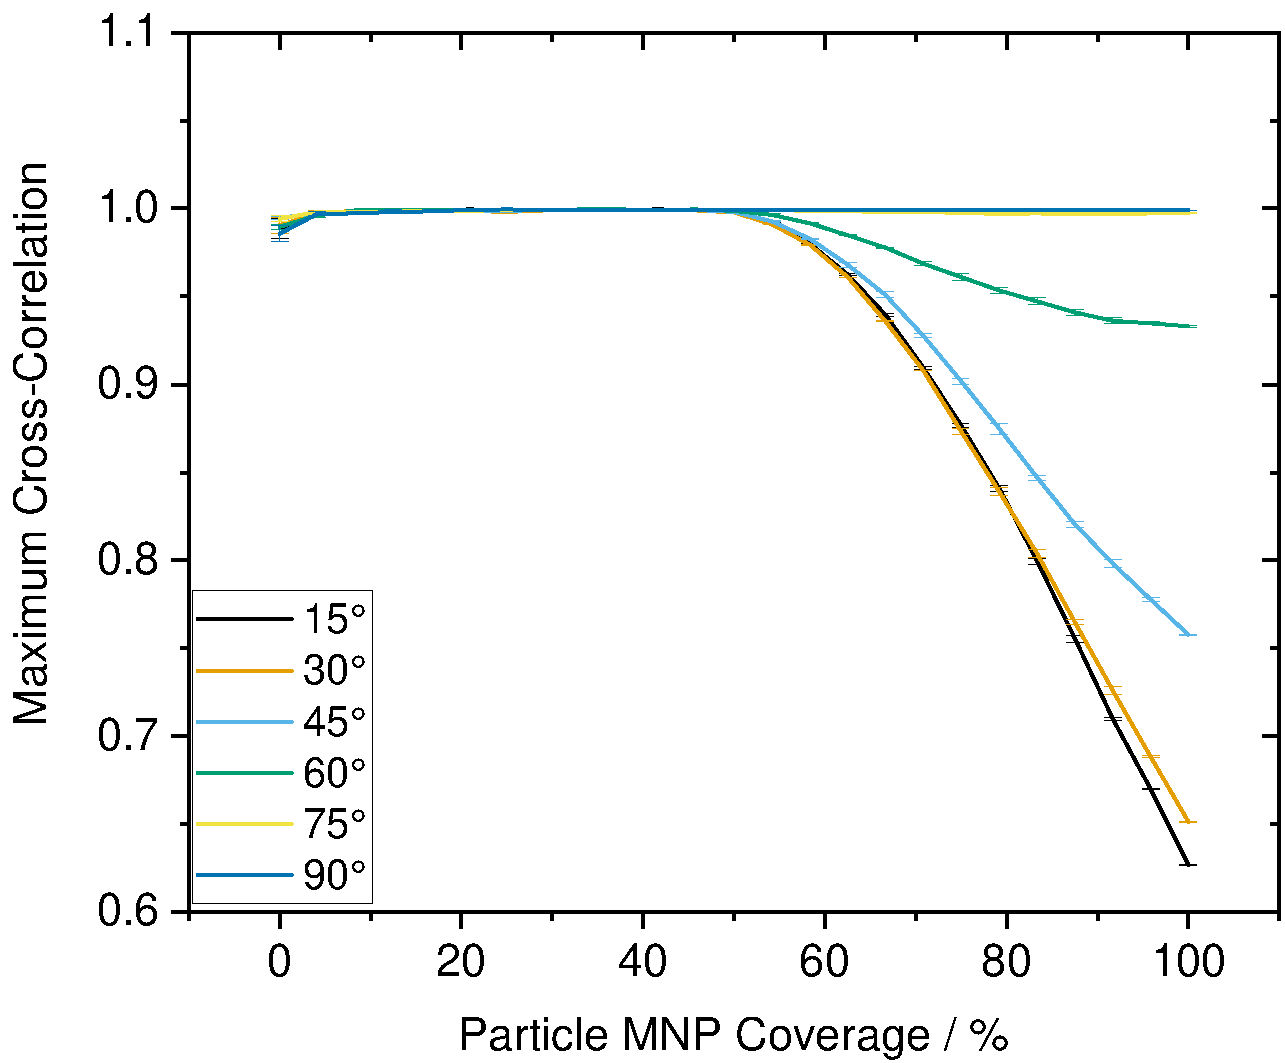
\includegraphics[width=.7\linewidth]{Ressources/Simulation/Aggregates}	
	\capption{Signal Correlation between Two-Cell Aggregates At Shifting Angles}{Two-Sphere aggregates are covered with \SI{200}{\nano\meter} \glspl{mnp} and simulated flowing over the sensor at differing respective angles. The \gls{sem} indicates a difference in cross-correlation of three truly random \gls{mnp} distributions. For low yaw angles and high coverages, the aggregate's signal reflects rather two single dipoles in superposition than one quite homogeneous dipole. This causes a high signal deviation from the reference and thus a low degree of correlation.}
	\label{fig:sim:aggregates}
\end{figure}
\clearpage

\section{The MRCyte Simulation Framework}
In this work, also a analytical simulation framework that is capable of simulating the synergy of multiple microfluidic effects was developed. The comprehensive framework features magnetic, fluid dynamic and biochemical processes inside the utilized microfluidic channel which act on a particle. Foremost, material parameters was stored inside the ``MRCyte'' class, which range from channel and particle properties to binding and friction constants. Basic velocity, shear and magnetic field computations build the core of the presented program. Additionally, several dimensionless parameters such as the Stokes or \gls{re} or particle properties can be computed.\\
With that, simulations of the fluid dynamics that influence a single microbead as well as force-equilibrium computations for the same bead were carried out. 

\todo{Capabilities - Simulation bead over sensor, particle distribution on surface, analysis of GMRTool data single and differential, magnetic field permanent}

\subsection{Fluid Fields inside the Microchannel}
The simulation framework provided a quantitative generation of the Hagen-Poiseuille flow profile inside the microchannel with the numerical solution of \cref{eq:flowRateRect}. The simulated channel had dimensions (w x h x L) \SI{700}{\micro\meter} x \SI{150}{\micro\meter} x \SI{15800}{\micro\meter}. The flow rate was chosen at \SI{80}{\micro\liter\per\minute}.\footnote{in accordance with the experimentally determined value} Tubing as well as time dependent effects were neglected. \\
The simulated \acrfull{u} for the whole channel cross-section can be observed in \cref{fig:sim:flowShear:vel:full}. Due to the no-slip boundary condition, \gls{u} is zero on the margin while the maximum of is reached in the geometric center. \gls{umean} in the channel ensues \SI{12670.84}{\micro\meter\per\second}. \\
In contrast, computation of the flow gradient in vertical direction and scaling with \gls{eta} yield the shear stress field.(\cref{fig:sim:flowShear:shear:full}) As the curvature of \gls{u} is zero in the channel center and maximal at the edges, the shear stress reaches highest values symmetrically at the horizontal edges of the channel.\footnote{Because the horizontal components of the gradients were neglected graceless} Resulting, the net viscous shear $\boldsymbol{\tau}_{viscous} = \frac{\partial u}{\partial z}$ cancels out over the whole channel cross-section.

Additionally, \gls{u} and \gls{tau_v} acting on a \SI{8}{\micro\meter} diameter bead on the channel bottom were analyzed.(\cref{fig:sim:flowShear:vel:particle,fig:sim:flowShear:shear:particle}). In the proximity to a wall and due to the applied boundary conditions, \gls{tau_v} enclosed by the bead surface is non-linear. Thus, the mean fluid velocity exposed to the bead amounts in $\overline{\mathbf{u}_{p}}$ =  \SI{2241.59}{\micro\meter\per\second}, whereas  $\overline{\boldsymbol{\tau}_{viscous,\, p}}$ strains with \SI{4.93}{\dyne\per\square\centi\meter}.

\begin{figure}[htb!]
	\centering	
	\subfloat{
		\subfigimg[height=135 pt]{a}{Ressources/Simulation/Flow/150um_vel}	%[width=\linewidth
		\phantomsubcaption
		\label{fig:sim:flowShear:vel:full}
	} \hfill
	\addtocounter{subfigure}{-1}
	\subfloat{
		\subfigimg[height=135 pt]{b}{Ressources/Simulation/Flow/150um_vel_particle}			
		\phantomsubcaption
		\label{fig:sim:flowShear:vel:particle}
	} \\
	\addtocounter{subfigure}{-1}
	\vspace{\baselineskip}
	\subfloat{
		\subfigimg[height=135 pt]{c}{Ressources/Simulation/Flow/150um_shear_chan}					
		\phantomsubcaption
		\label{fig:sim:flowShear:shear:full}
	} \hfill
	\addtocounter{subfigure}{-1}
	\subfloat{
		\subfigimg[height=135 pt]{d}{Ressources/Simulation/Flow/150um_shear_part}					
		\phantomsubcaption
		\label{fig:sim:flowShear:shear:particle}
	}
	%	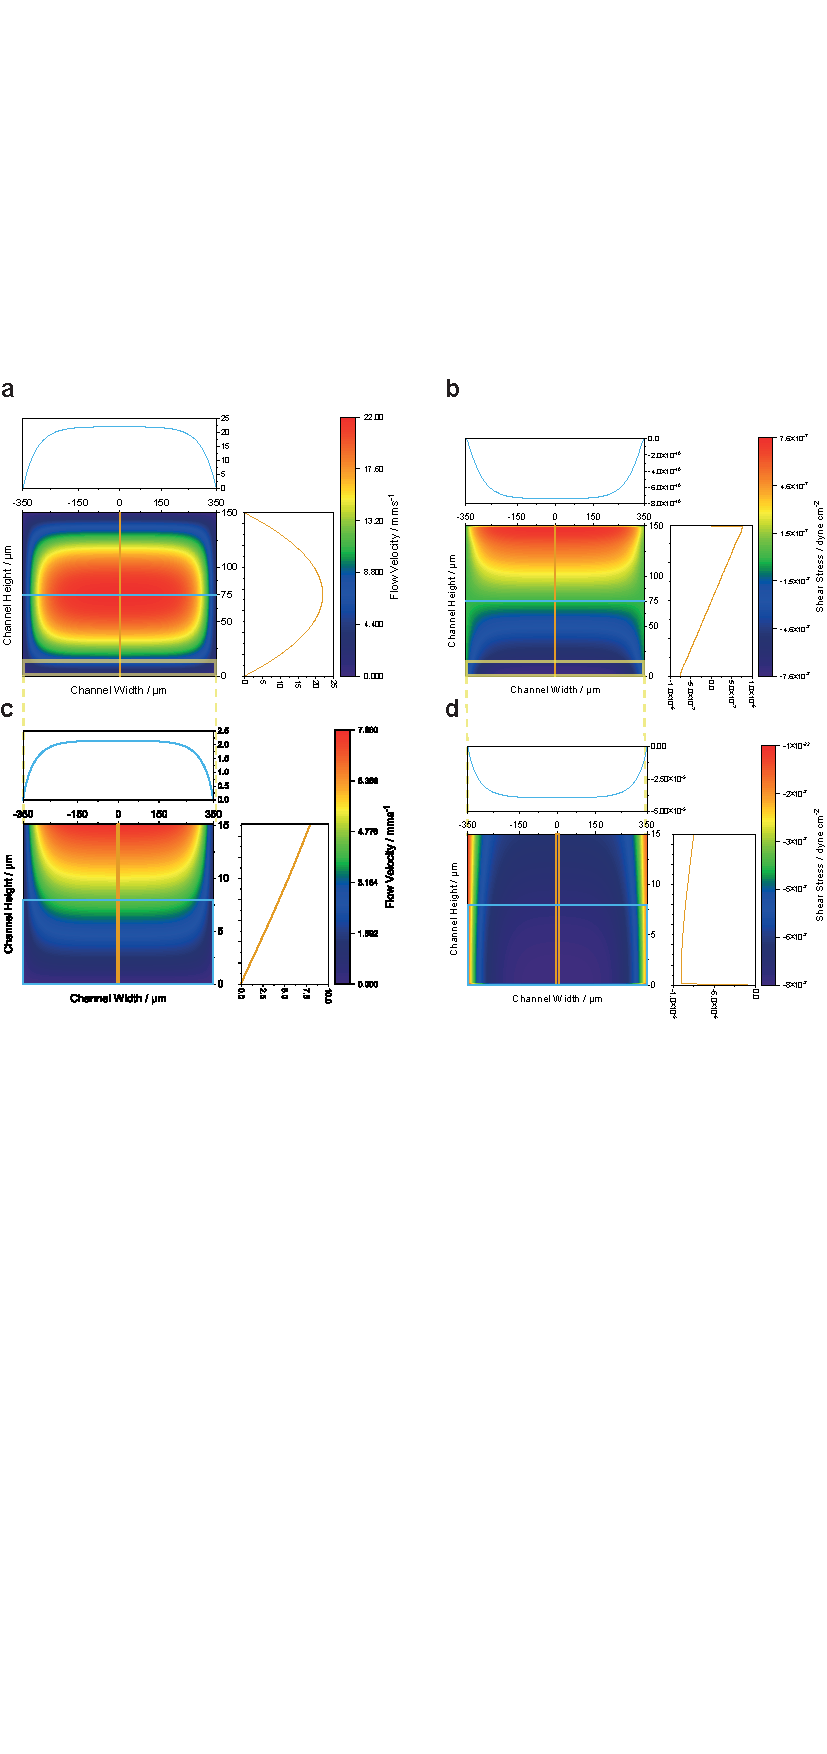
\includegraphics[width=\linewidth]{Ressources/Simulation/FlowShearFigure}
	\capption{Flow Field and Shear Stress Simulation of the utilized Microchannel}{Flow (\textbf{a}) and vertical shear (\textbf{c}) field inside the microchannel with dimensions (w x h x L) \SI{700}{\micro\meter} x \SI{150}{\micro\meter} x \SI{15800}{\micro\meter} for a flow rate of \SI{80}{\micro\liter\per\minute} and with neglected tubing effects. The subplots on the right and top side show the mean horizontal and vertical profile in \SI{0}{\micro\meter} width and \SI{75}{\micro\meter} height, respectively. (vertical: \blueline, horizontal: \orangeline) Due to the no-slip condition, the velocity at the walls equals zero and the shear is maximal. The maximum of the Hagen-Poiseuille profile is located in the channel center. Over the cross-section the mean flow velocity $\overline{\mathbf{u}}$ equals \SI{12670.83}{\micro\meter\per\second}. Resultingly, the net horizontal viscous shear  $\boldsymbol{\tau}_{viscous} = \frac{\partial u}{\partial z}$ cancels out over the whole channel cross-section. \\
	Flow (\textbf{d}) and vertical shear (\textbf{d}) field acting on a \SI{8}{\micro\meter} diameter bead on the channel bottom. The mean fluid velocity trapped by the bead profile results in  $\overline{\mathbf{u}_{p}}$= \SI{2241.59}{\micro\meter\per\second}, whereas the viscous shear strains with $\boldsymbol{\tau}_{viscous}$ = \SI{4.93}{\dyne\per\square\centi\meter} }
	\label{fig:sim:flowShear}
\end{figure}
\clearpage

\subsection{Modelling the Force-Equilibrium of a Rolling Bead over a Biofunctionalized Surface}
\todo{nice intro}
With the supplier's parameters of a \SI{8}{\micro\meter} micromer-M bead (micromod Partikeltechnologie GmbH, Rostock) the corrected drag force on a bead on the bottom of the standard utilized microchannel resultes in \SI{463.65}{\pico\newton} for \SI{80}{\micro\liter\per\minute}.\\
If the bead was functionalized with biotin under negligence of the differential equations for the association constants, the number of interacting groups would result in the present surface charges. Surface charge density resultes in \SI{1}{\micro\mole\per\gram} of \gls{carboxyl} and \gls{amine} beads as of the supplier's datasheet. Hence, a fully saturated bead is covered in \num{177500} biotin molecules.\\
The streptavidin coverage of the channel floor was modeled in excess over the biotin ligands. The penetration depth was estimated by the size of several monolayers protein. As described by \citet{lit:fluidic:ModelMIT}, an approach of \SI{30}{\nano\meter} is a reasonable quantity. In turn, the surfaces were in contact with \SI{1.51}{\micro\meter\squared} which constitutes \SI{0.75}{\percent} of the \SI{8}{\micro\meter} bead surface. This reveals that \num{1329} biotin molecules can interact with the floor. A summation of the \gls{f:protein} at \SIrange{5}{150}{\pico\newton} per streptavidin-biotin bond yields the resulting adhesion force with a magnitude of \SIrange{6.7}{199}{\nano\newton}.\cite{lit:bio:biotin:rupture} 

The binding force is in the same range as the perpendicular magnetophoretic force caused by the permanent magnet under the sensor chip ($\nabla \mathbf{B}$ = \SI{10}{\tesla\per\meter}) as well as by the nickel-iron chevron structures on the chip ($\nabla \mathbf{B}$ $\approxeq$ \SI{5}{\kilo\tesla\per\meter}). Clearly, in the near-field approximation the nickel-iron structures dominate \gls{f:mag} (\cref{eq:f:mag}). With the manufacturer given saturation momentum of one particle (\SI{1.12}{\pico\ampere\meter\squared}), the magnetic attraction force eventuates in \SI{5.6}{\nano\newton}.

\begin{align}
	\mathbf{F}_\parallel = \mathbf{F}_{drag} - C_{rr} \cdot (\mathbf{F}_{mag} \ +\ \mathbf{F}_{protein}  \ +\ \mathbf{F}_{grav}\ -\ \mathbf{F}_{shear} ) \label{eq:f:balance} \\
	C_{rr} = \sqrt{\frac{\text{z}}{d}} = \sqrt{\frac{\SI{30}{\nano\meter}}{\SI{8}{\micro\meter}}} = 0.0612 \label{eq:corr:roll}
\end{align}

In order to merge this analytic force balance, all remaining forces have to be projected into the direction of \acrfull{f:drag}.(\cref{eq:f:balance}) This is achieved by the introduction of the \gls{corrRoll} for a perfectly elastic surface.(\cref{eq:corr:roll}) In a first order approximation, the factor depends only on the \acrfull{z} and the bead diameter ($d$). However, scientific literature about the rolling resistance of microbeads on microfluidic or protein covered surfaces does not exist yet to confirm this macroscopic factor for the microscale. \\
Scaling all orthogonal forces to the \acrlong{f:drag} with \gls{corrRoll} yields a net positive result (\SI{154.08}{\pico\newton}) for an unfunctionalized surface (\gls{f:protein} $\overset{!}{=}$ \num{0}) which indicates a rolling motion in flow direction. Notwithstanding, above a critical interaction number of \numrange{16}{503} biotin-streptavidin bonds - for the respective release forces of \SIrange{5}{150}{\pico\newton} per linkage - the particle resists \acrlong{f:drag} and adheres to the surface.

This behavior will be exploited in further measurements for ``bead loss experiments'' in order to measure a concentration difference with different degrees of biotinylated beads.


\clearpage
\section{Reference Bead Surface Functionalization}
After simulation of their respective coverages, biotin was titrated on \SI{8}{\micro\meter} reference beads with two different surface terminations in order to selectively bind \glspl{mnp} with the counter-agent streptavidin to the surface. First, \gls{amine}-microbeads were modified by sulfo-NHS-biotin. Second, \gls{carboxyl}-beads were coated by amine-PEG$_2$-biotin via EDC-NHS-activation. On the same beads Anti-IgG1-PE antibodies were titrated after the same coupling chemistry.\\
Subsequently, biotin-coated beads were analyzed in the flow cytometer in the by staining with Atto-488 (Ex: \SI{500}{\nano\meter}, Em: \SI{520}{\nano\meter}) coupled streptavidin. The antibody was already industrially modified with \gls{pe} and measured at \SI{488}{\nano\meter} excitation and \SI{585}{\nano\meter}  emission wavelength. The gating was standardized by the strategy found in \cref{sec:meth:beadCharact}, \cref{fig:gatingstrategy-layout}. Subsequently, the \gls{mfi} was computed and fitted with a Hill-function.(\cref{eq:hill}) Stability of carboxylated and aminated beads and subsequently their respective modification protocols was evaluated for \SI{12}{days}.


\subsection{Amine-Surface Biotinylation}
As first approach, polystyrene copolymer microbeads with \SI{8}{\micro\meter} diameter were functionalized by (sulfo-)NHS-biotin after a standard protocol. A titration of the biotin reactant yielded a varying surface coverage as shown in \cref{fig:biotinyl:titration:nh2}. During this one-pot-reaction, the water-soluble sulfo-NHS-biotin forms an \gls{amide} linkage with the primary \gls{amine} and \iupac{1-\-hydroxy\--2,5-\-dioxo\-pyrrolidine-\-3-\-sulfonate} splits off as byproduct.\\
As can be seen from the \gls{sem} error-bars from the plot \ref{fig:biotinyl:titration:nh2}, which were constructed from three true biological replicates, this process is highly reproducible. Therefore, an surface coverage in different grades of biotinylation could be obtained accurately with a \gls{rsquadj} of \num{0.981} for the resulting Hill fit (\orangedash).

\begin{figure}[h]
	\centering
	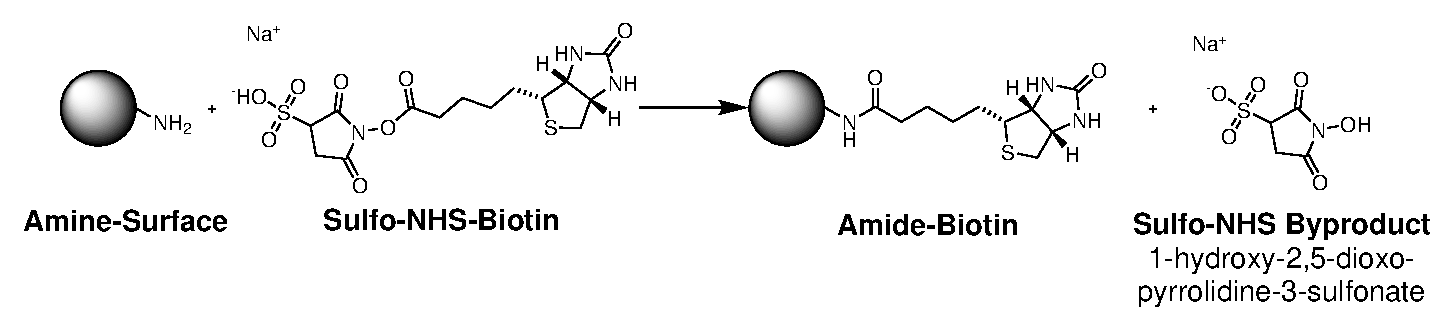
\includegraphics[width=\linewidth]{./Ressources/Chemistry/Sulfo-NHS.eps}
	\capption{Amine Bead Modification with Sulfo-NHS-Biotin}{An amine terminated bead brought into reaction with sulfo-NHS-biotin. Both form an amide linkage and bind biotin covalently to the surface. As byproduct the sulfo-NHS-ester splits off.}
	\label{fig:Chem:NH2-NHS}
\end{figure}

\clearpage

\begin{figure}
	\centering
	\subfloat{
		\subfigimg[height=95pt]{a}{./Ressources/Biotinyl/mag-nh2}	
				\phantomsubcaption
		\label{fig:biotinyl:titration:nh2}
	} \hfill
	\addtocounter{subfigure}{-1}
	\subfloat{
		\subfigimg[height=95pt]{b}{./Ressources/Biotinyl/cooh}	
		\phantomsubcaption
		\label{fig:biotinyl:titration:cooh}
	}\hfill
	\addtocounter{subfigure}{-1}
	\subfloat{
		\subfigimg[height=95pt]{c}{./Ressources/Biotinyl/IgG-cooh}	
		\phantomsubcaption
		\label{fig:biotinyl:titration:igg}
	} \\
	\addtocounter{subfigure}{-1}
	\vspace{\baselineskip}
	\subfloat{
	\subfigimg[width=.7\linewidth]{d}{./Ressources/Biotinyl/stability}
	\phantomsubcaption
	\label{fig:biotinyl:titration:stability}	
	}

	\capption{Titration of Biofunctional Molecules on \SI{8}{\micro\meter} Particles}{ Titration curves of NHS-biotin (\textbf{a}), Amin-PEG$_2$-Biotin (\textbf{b}), and Anti-IgG1 (\textbf{c}) with their respective Hill fits. The corresponding fit parameters as well as the goodness factor are shown in \cref{tab:biotinyl:fitParams:beads}. (\textbf{d}) Stability analysis of functionalized \gls{carboxyl} and \gls{amine} beads over \SI{12}{days}. The carboxylate particles show a exponential decrease with a half-life of \SI{1.43}{days} as determined by the exponential fit. The respective parameters are shown in \cref{tab:biotinyl:fitParams:stability}.}
	\label{fig:biotinyl:titration}
\end{figure}
\begin{table}[!h]
	\subfloat[  ]{
		\begin{tabularx}{.6\linewidth}[t]{cccc}
			\toprule[1.2pt]
			Param. & Hill \ref{fig:biotinyl:titration:nh2} & Hill \ref{fig:biotinyl:titration:cooh} & Hill \ref{fig:biotinyl:titration:igg} \\
			\midrule
			$V_{max}$ &   \num{175.21619} & \num{140.39153} & \num{713.83643}  \\
			$k$ & \num{57.36713}  & \num{4.12661}  & \num{182.83011} \\
			$n$ &  \num{1.47488} & \num{1.07493} &  \num{0.72458}\\
			\Gls{rsquadj} & \num{0.98121}  & \num{0.99722}  & \num{0.99226}  \\
			\bottomrule
		\end{tabularx}
		\label{tab:biotinyl:fitParams:beads}
	}%
	\hfill
	\subfloat[  ]{
		\begin{tabularx}{.25\linewidth}[t]{cc}
			\toprule[1.2pt]
			Param. & Exp. \ref{fig:biotinyl:titration:stability} \\
			\midrule
			$A$ &   \num{0.91263} \\
			$\tau_{decay}$ & \num{1.42557}  \\
			$y_0$ & \num{0.12369}  \\
			\Gls{rsquadj} & \num{0.96655} \\
			\bottomrule
		\end{tabularx}	
		\label{tab:biotinyl:fitParams:stability}
	}
	\capption{Fit Parameters of Biotinylation}{(\textbf{a}) Coefficients for the Hill fits in \cref{fig:biotinyl:titration:nh2,fig:biotinyl:titration:cooh,fig:biotinyl:titration:igg} (\textbf{b}) Exponential fit coefficients for the stability analysis in \cref{fig:biotinyl:titration:stability}}
	\label{tab:biotinyl:fitParams}
\end{table}
\clearpage

\subsubsection{Carboxylate-Surface Functionalization}
In a second approach, particles with opposite partial surface charge, mediated through \gls{carboxyl} groups, have been functionalized. In turn, particles were pre-activated in \gls{edc} and \gls{nhs} in \gls{mes}/\gls{mest} buffer. There are two distinct reasons for the usage of \gls{mes} based buffers rather than \gls{pbs} or \gls{macs}. First, \gls{edc} has its reactive maximum at \pH\ \numrange{5}{6}. Second, buffers containing primary \glspl{amine} (TRIS / glycine) or \glspl{carboxyl} (acetate / citrate) will quench the reaction and therefore limit the efficacy.\\
Afterwards, the beads were washed carefully and incubated with \gls{amine}-\acrshort{peg}$_2$-biotin. Here, \gls{peg} indicates a hydrophilic spacer arm between both functional groups and in this case has length of a two units. The full functionalization procedure is explained in more detail in \cref{fig:chem:COOH-EDC-NHS}. 

As shown in \cref{fig:biotinyl:titration:cooh}, particles were functionalized equally compared to \gls{amide} surfaces. However, the stability of \gls{carboxyl} particles yields \SI{1.43}{days} half-life in a continuous measurement over \SI{12}{days} with a subsequent exponential fit. Additionally, both procedures show an outlier at high concentrations which could not be explained during the course of this thesis. 

Third, \gls{carboxyl}ated particles have been also functionalized with the Anti-IgG1-\gls{pe} antibody. Again, a Hill-shaped titration curve was achieved, but due to the costly reagent a saturated surface coverage was not reached. (\cref{fig:biotinyl:titration:igg}) \\
Therefor, the fit curve has to be interpreted cautiously. Although it converged and represents the data with an \gls{rsquadj} of \SI{99.2}{\percent}, the goodness of fit determined by the reduced $\chi^2$ statistic results in a value of \num{278.1} which indicates an underestimation of the error variance.

\clearpage
\section{Concentration Measurements in MRCyte}
Driving factor for the concentration measurement is the absolute count of immunomagnetically labeled cells in diluted or whole blood which is not possible in today's optics-based devices due to the excess of \glspl{rbc}.\cite{lit:bio:Alberts} Therefore, with the in \cref{sec:theo:magnet} described sensor setup, absolute concentrations of magnetic reference beads were attempted to measure.\\
Consequently, beads with acrylate surface were pumped through a microfluidic channel with a permanent magnet underneath. The magnet drew every magnetic particle to the ground, where they were focused on the sensor bridge and subsequently measured there. From the received signal several parameters such as peak amplitudes, locations, zero-crossings, and relative distances between each other were computed. (\cref{fig:conc:example}) However, for a concentration measurement mostly the correct detection of a signal from the noisy stream or from a superposition of multiple simultaneously measured particles was critical. The related error sources and countermeasures will be elaborated in \cref{sec:res:Correction}.

\begin{figure}[b]
	\centering
	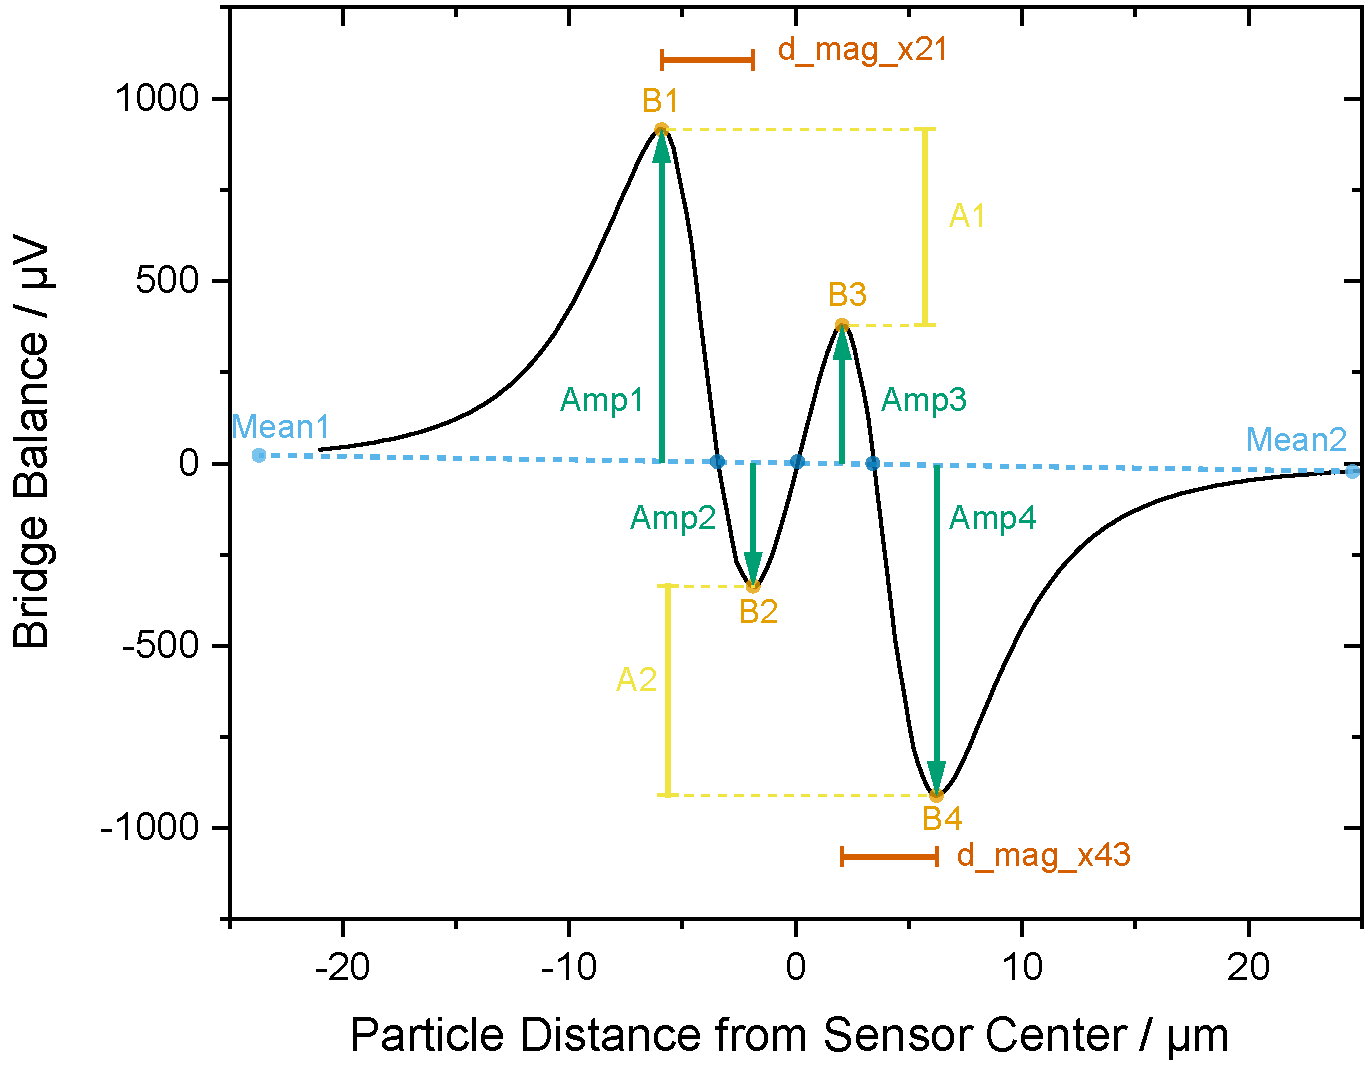
\includegraphics[width=.7\linewidth]{Ressources/Simulation/ExampleSignal}
	\capption{Example Signal of Magnetic Measurement}{Signals generated from the Wheatstone bridge sensor setup feature a certain shape which allows for several measures. In case the overall signal stream carries a constant or linear offset, it is scaled to the means before and after the detected peak pattern. (\textcolor{OlightBlue}{Mean1, Mean2}) The x- and y-positions of each peak are denominated by \textcolor{Oorange}{B1-4} and \textcolor{Ogreen}{Amp1-4}, respectively. The crossings of the signal through the linear connection of both means are denominated by \textcolor{OdarkBlue}{n1-3} (in the figure by \darkBlueCircle). Further, the difference between the equally oriented peaks \textcolor{Oorange}{B3}-\textcolor{Oorange}{B1} and \textcolor{Oorange}{B4}-\textcolor{Oorange}{B2} give a measure for the homogeneous movement of the measured object and are called \textcolor{Oyellow}{A1} and \textcolor{Oyellow}{A2} each. From these values the overall velocity $v$ can be approximated because the \gls{dgmr} and \gls{fs} is fixed precisely. Analogously, the magnetic diameter of a dipole is computed by the mean of the differences \textcolor{Oorange}{B2}-\textcolor{Oorange}{B1} and \textcolor{Oorange}{B4}-\textcolor{Oorange}{B3}.}
	\label{fig:conc:example}
\end{figure}

By measuring the absolute concentration with a commercially available flow cytometer (MacsQuant 10, Miltenyi), a reference bead count was established. In a pre-test, beads were taken directly from the microcentrifuge tube, after pumping through a syringe, and after pumping through a syringe with \SI{10}{\centi\meter} of connected through tubing (ID \SI{0.5}{\milli\meter}, RS Chemicals). Afterwards, they were counted in the flow cytometer in equal volumes. Additionally, two different buffers - \gls{macs} and \gls{pbs} - and two different surface terminations were used. Both buffers are based on \acrfull{pbs}. Notwithstanding \gls{macs} contains \gls{edta} as chelator for divalent ions, Tween 20 - a non-ionic surfactant -, and an azide-based stabilizer. Hence, the wetting of surfaces and the electrostatic interactions of these buffers differ. The same properties were varied on the bead surface by choosing acrylate- and biotin-terminated beads.\\
In \cref{fig:conc:losses_syringe}, a trend (without statistical confidence) can be observed that shows a decrease in particle counts after every additional surface which beads could potentially interact with. In term, a correct count in absolute numbers seems out of range. However, a calibration of the system with the flow profile inside the channel to compensate for losses subjected to connectors and magnetic enrichment structures was carried out successfully.
\begin{figure}[b]
	\centering
	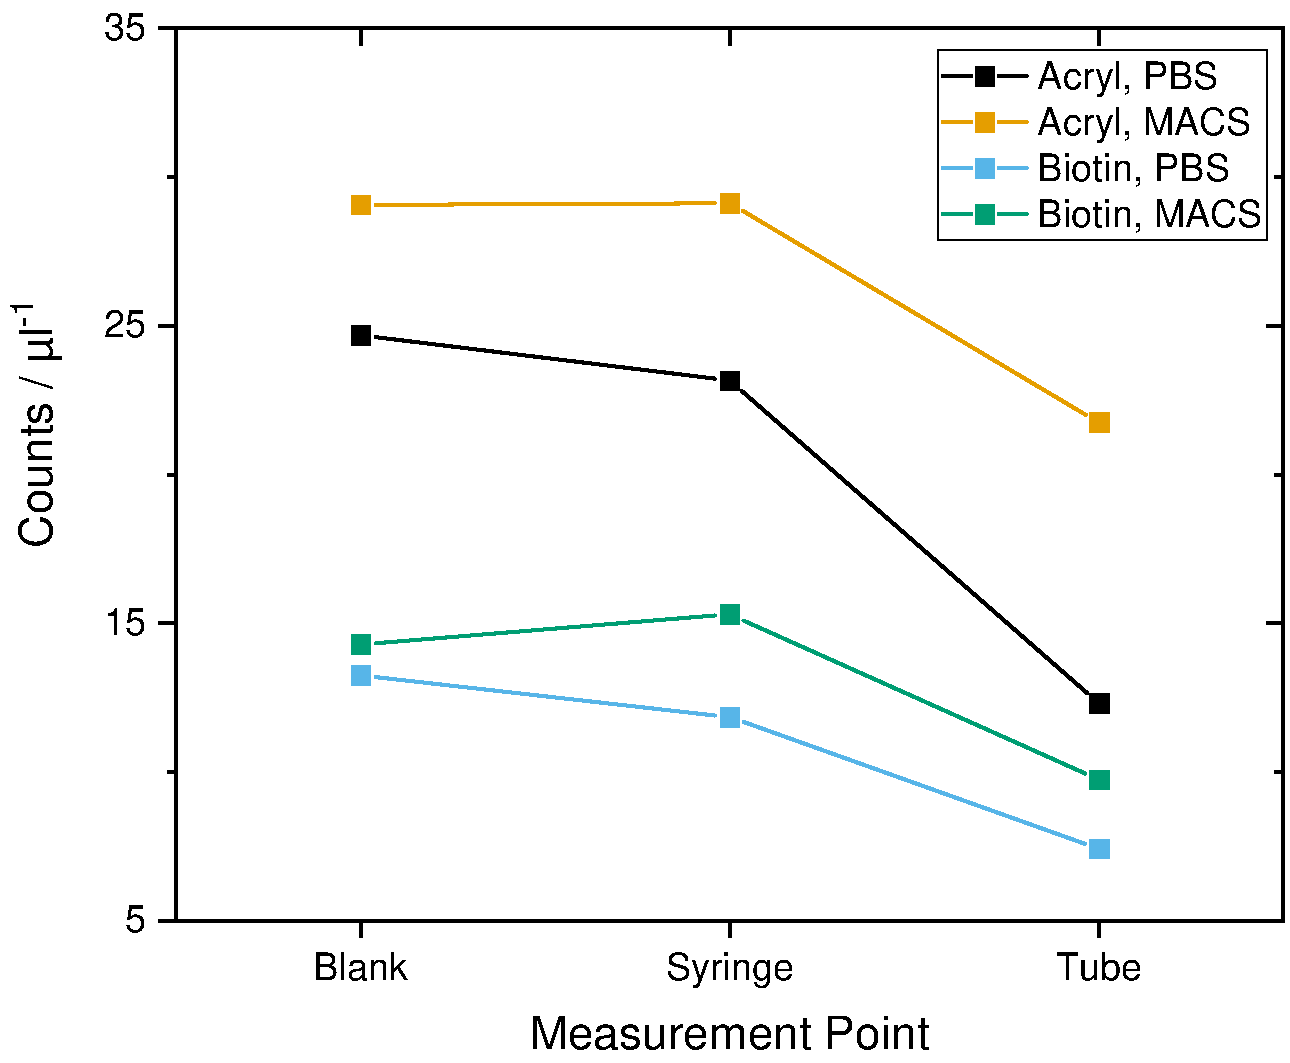
\includegraphics[width=.7\linewidth]{Ressources/Concentration/Losses-Syringe-Tubing}
	\capption{Bead Loss Evaluation in Connectors}{Bead concentrations measured in equal volumes in the flow cytometer after being pumped through a syringe or a syringe with connected tubing. The blank sample was measured directly from the stock solution. Additionally, electrostatic and surface tension related effects were resolved by the usage of different buffers and bead surfaces.}
	\label{fig:conc:losses_syringe}
\end{figure}


\clearpage
\subsection{Measurement Error Sources and Calibration of Flow Field}
\label{sec:res:Correction}
In order to account for the bead losses due to the tubing connectors, the Hagen-Poiseuille flow profile, and magnetophoretic enrichment structures, the measured bead concentration was corrected in two different approaches.(\cref{eq:corr:conc}) On the one hand side, the typical assay correction to the ground truth by a constant \gls{corrConst} computed from the blank population was established. On the other side, a \gls{corrVel} compared the \acrfull{umean} to the \gls{vc}.
\begin{equation}	
	c_{beads,\, expected} = c_{beads,\, measured}  \cdot C \label{eq:corr:conc}
\end{equation}
The \gls{corrConst} relates a reference count in the optical flow cytometer to the measurement in the magnetic flow cytometer.(\cref{eq:corr:const}) Equally-adjusted bead concentrations in the samples allow for a correction to the reference system. However, for an assay usage the initial concentration of beads either has to be known precisely or has to be irrelevant, for example in regards of a standardized measurement procedure. Besides, \gls{corrConst} provides a reliable and generalizable option for correction. 
\begin{align}
	C_{const} &= \frac{c_{beads,\, standard\ procedure}}{c_{beads,\, MRCyte}} \label{eq:corr:const}\\
	v_c &= 2\ d_{gmr} \frac{f_s}{n_3-n_1} \label{eq:v:c} \\
	C_{velocity} &= \frac{\overline{\mathbf{u}}}{v_c} = \frac{Q}{A \cdot v_c} \label{eq:corr:vel} 
\end{align}
\begin{figure}[b]
	\centering
	\subfloat{
		\subfigimg[height=150pt]{a}{Ressources/Concentration/BiotinylWrongCorrection}
		\phantomsubcaption
		\label{fig:conc:BiotnylWrongCorr:velConst}	
	} \hfill
	\addtocounter{subfigure}{-1}
	\subfloat{
		\subfigimg[height=150pt]{b}{Ressources/Concentration/BiotinylTime}	
		\phantomsubcaption
		\label{fig:conc:BiotnylWrongCorr:time}
	}
	\capption{Error Sources in Concentration Measurements}{(\textbf{a}) Robustness evaluation of the both correction factors \gls{corrConst} and \gls{corrVel} for protein coated surfaces. The mean and \gls{sem} of plain and biotinylated measurements show a high deviation from physically reasonable expections when corrected for the velocity (right). In contrast, \gls{corrConst} can intrinsically correct only well below \SI{100}{\percent}. (\textbf{b}) Mean and \gls{sem} of a fit-corrected bead capture experiment with several error sources. Initially, the magnetophoretic structures have to be filled and thus decrease the plain count for the first \SI{100}{\micro\liter}. (\orangeline) Additionally, the high deviation offsets the correction factor so that the stable measurement from \SIrange{100}{200}{\micro\liter} lies now above the ideal reference. In contrast, the biotinylated beads are captures by the surface functionalization and hence a very low concentration is measured. However, a steep rise with pulsations can be observed when the surface is saturated with beads and the particles begin to flow over the sensor in bursts. (\blueline) The abrupt decline to the end of the measured volume is most probably related to sedimentation effects inside the emptying syringe.}
	\label{fig:conc:BiotnylWrongCorr}
\end{figure}
The \gls{corrVel} relates the effective particle velocity to the total fluid velocity in order to eradicate flow profile provoked effects.(\cref{eq:corr:vel}) Whereas \gls{umean} was determined by \acrfull{q} through a cross-sectional \gls{a} of the channel, \gls{vc} was analyzed from the measured signal stream. Here, the intrinsic \acrfull{dgmr} was divides by the time difference where the bead passed exactly over a \gls{gmr}-element.(\cref{eq:v:c}) These specific timepoints are visible as dimensionless zero-crossings $n_1$ and $n_3$ in the signal and can be converted by scaling with the \acrfull{fs} into the time domain. \\
However, if the bead velocity is not solely dependent on fluid dynamic effects - especially in the light of surface functionalizations - \gls{corrVel} can not be applied to experiments robustly. This is depicted in a sample experiment with a protein covered surface in \cref{fig:conc:AbsConcError:concerror}. By definition, the \gls{corrConst} can not be well above than \SI{100}{\percent} whereas the count correction by \gls{corrVel} differs by \SI{600}{\percent} through variations in the velocity measurement. 

An adaptation of these corrections to real measurements are depicted in \cref{fig:conc:AbsConcError}. 


\begin{figure}[b!]
	\centering
	\subfloat{
		\subfigimg[height=150pt]{a}{Ressources/Concentration/ConcentrationError}	
		\phantomsubcaption
		\label{fig:conc:AbsConcError:concerror}
	} \hfill
	\addtocounter{subfigure}{-1}
	\subfloat{
		\subfigimg[height=150pt]{b}{Ressources/Concentration/ConcentrationVelocity}	
		\phantomsubcaption
		\label{fig:conc:AbsConcError:experimental}
	}
	\capption{Absolute Concentration Measurements}{Mean of 3 true biological replicates (\textbf{a}) mean, sd (\textbf{b}) mean, SEM, Reference Count based error: Linear fit steepness \num{0,34622 +- 0,00968} --> Correction Factor (inverse) \num{2,88833 +- 0,08075}, Velocity Based Correction: $Q/A$ Dims: \SI{700}{\micro\meter}x\SI{50}{\micro\meter} Q = \SI{30}{\micro\liter\per\minute} --> \num{2,26109}}
	\label{fig:conc:AbsConcError}
\end{figure}

\subsection{Count Stability}
Measurement over 1h

\begin{figure}[!h]
	\centering
	\subfloat{
		\subfigimg[height=150pt]{a}{Ressources/Concentration/BiotinylCountAll}	
	} \hfill
	\subfloat{
		\subfigimg[height=150pt]{b}{Ressources/Concentration/BiotinylTimeAll}	
	}
	\capption{Reproducibility of Concentration Measurements with Saturated Neutravidin Surface}{(\textbf{a}) \SI{80}{\micro\liter\per\minute} mean, SEM (\textbf{b}) All,mean, SEM,}
	\label{fig:conc:All}
\end{figure}



\begin{figure}
	\centering
	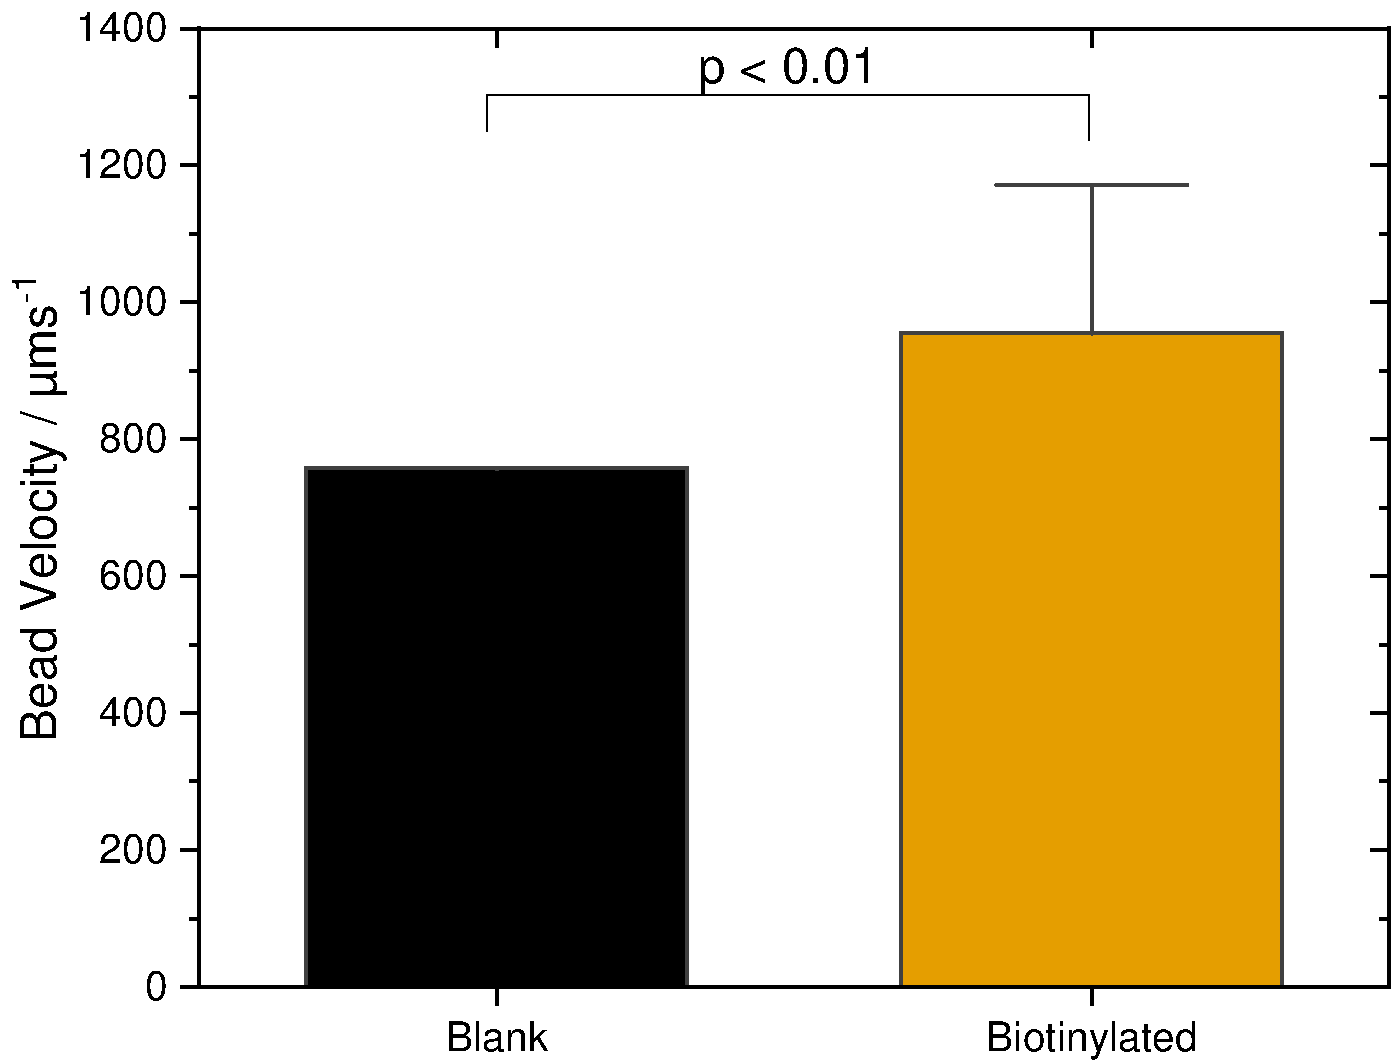
\includegraphics[width=.7\linewidth]{Ressources/Concentration/CaptureVelocity}
	\capption{Measured Bead Velocity}{ p < 0.01}
	\label{fig:conc:vel}
\end{figure}




\subsubsection{Concentration Measurement in Diluted Whole Blood}


\begin{figure}
	\centering
	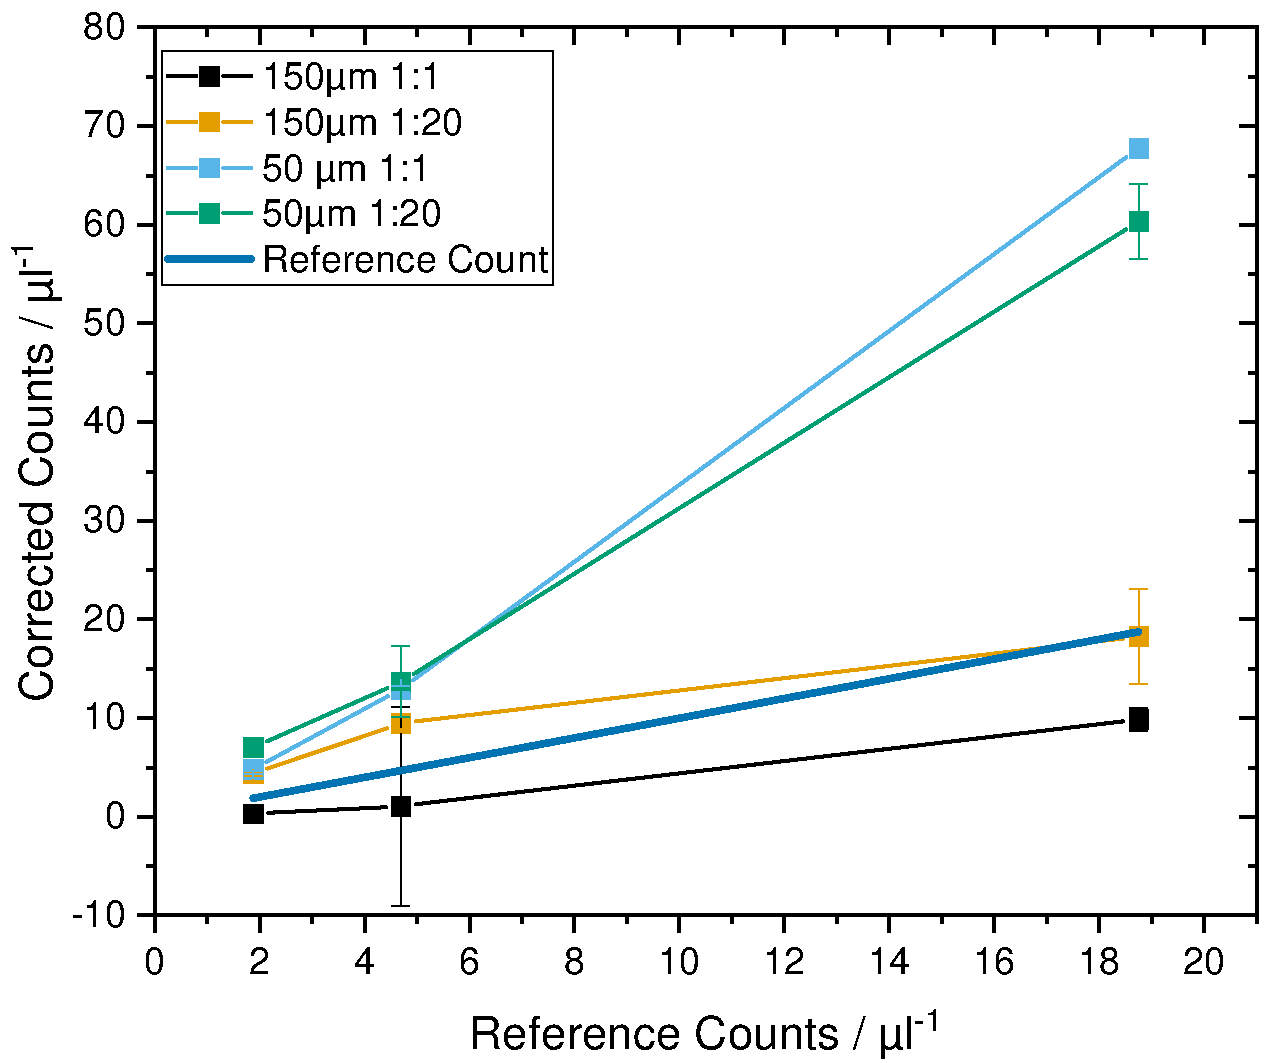
\includegraphics[width=.7\linewidth]{Ressources/Concentration/CorrectionBlood}
	\capption{Absolute Concentration Measurement in Blood Samples Under Varying Channel Height}{Velocity Correction does not work for high concentrations in \SI{50}{\micro\meter}}
	\label{fig:conc:blood}
\end{figure}




\subsection{Differential Counting Setup}

\subsubsection{Sensitivity Calibration}

\begin{figure}
	\centering
	\subfloat{
		\subfigimg[height=150pt]{a}{Ressources/Differential/Optupper}	
	} \hfill
	\subfloat{
		\subfigimg[height=150pt]{b}{Ressources/Differential/Optlower}	
	}
	\capption{Hysteresis Calibration for Stacked \Gls{pcb} }{(\textbf{a}) Optimized for top sensor (\textbf{b}) Optimized for bottom sensor}
	\label{fig:diff:sensitivity}
\end{figure}

\subsubsection{Concentration Measurement in Buffer Solution}



\begin{figure}
	\centering
	\subfloat{
		\subfigimg[height=150pt]{a}{Ressources/Differential/Bottom}	
	} \hfill
	\subfloat{
		\subfigimg[height=150pt]{b}{Ressources/Differential/Top}	
	}
	\capption{Flow Rate Dependency of Counting Setup}{(\textbf{a}) Optimized for top sensor (\textbf{b}) Optimized for bottom sensor}
	\label{fig:diff:flowRate}
\end{figure}

\begin{figure}
	\centering
	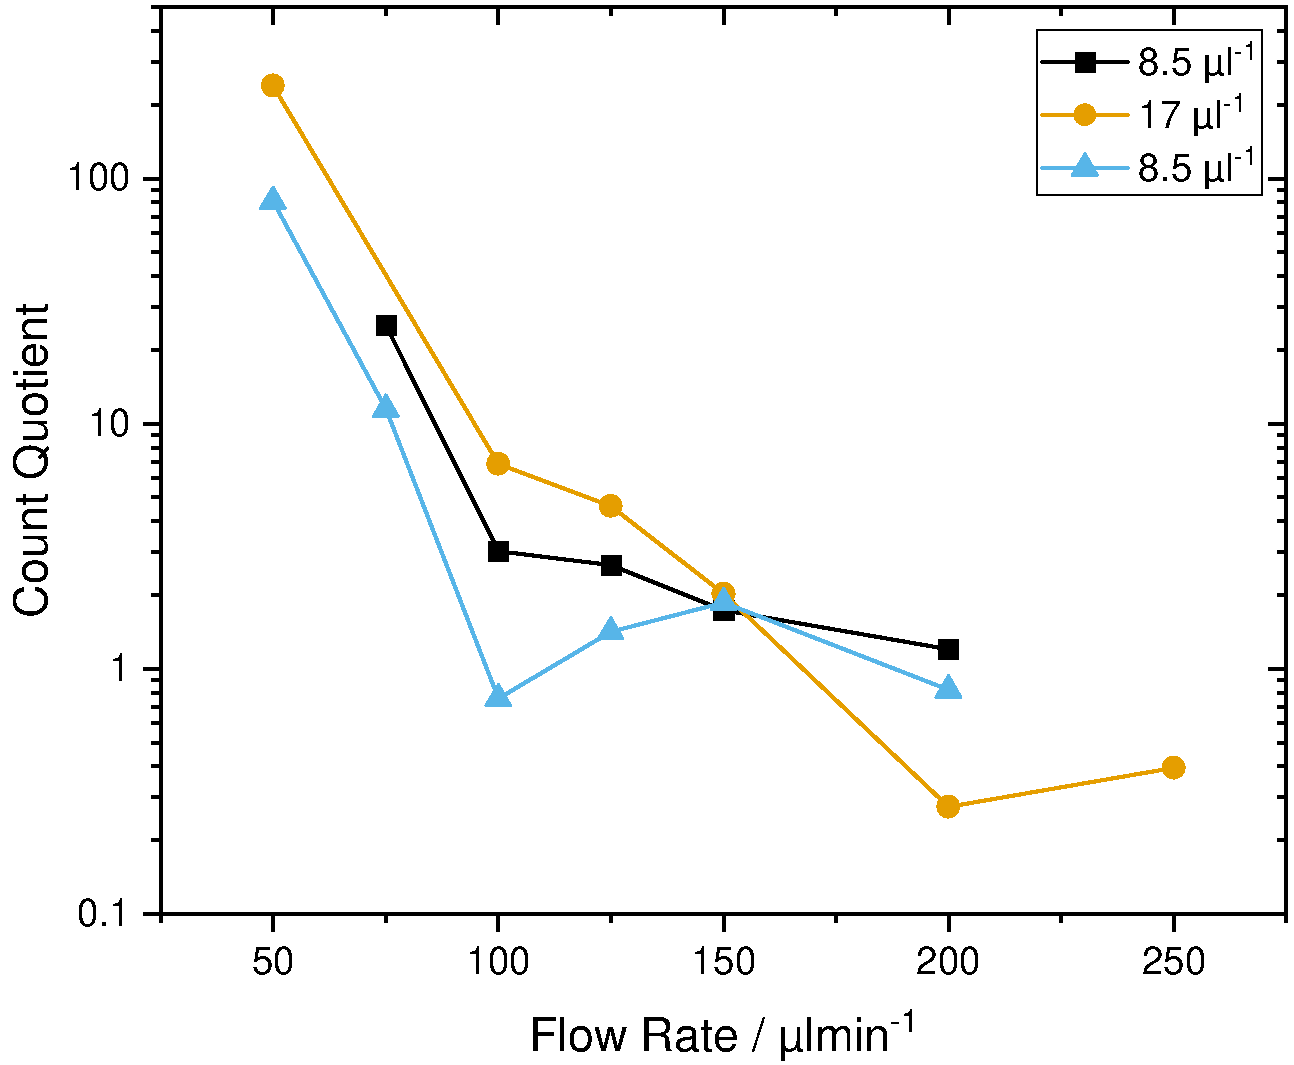
\includegraphics[width=.7\linewidth]{Ressources/Differential/Differential}
	\capption{Optimal Differential Counting Flow Rate}{Losses in different buffers and bead surfaces.}
	\label{fig:conc:optimum}
\end{figure}




\subsection{Surface Magnetization of Biofunctionalized Beads}

Somehow BNF-Dextran showed unspeficity initally, but not anymore later on

\begin{figure}
	\centering
	\subfloat{
		\subfigimg[height=150pt]{a}{Ressources/Concentration/BNFC1}	
	} \hfill
	\subfloat{
		\subfigimg[height=150pt]{b}{Ressources/Concentration/BNFVc}	
	}
	\capption{Bead Coverage Assay with BNF-Dextran-redF-\SI{100}{\nano\meter}}{(\textbf{a}) 1. \SI{80}{\micro\liter\per\minute} 2. \SI{40}{\micro\liter\per\minute} 3. \SI{20}{\micro\liter\per\minute} 4. \SI{10}{\micro\liter\per\minute} (\textbf{b}) d = \SI{8}{\micro\meter}}
	\label{fig:conc:BNF}
\end{figure}



\begin{figure}
\centering
\subfloat{
	\subfigimg[height=150pt]{a}{Ressources/Concentration/OceanC1}	
} \hfill
\subfloat{
	\subfigimg[height=150pt]{b}{Ressources/Concentration/OceanVc}	
}
\capption{Bead Coverage Assay with OceanNanotec \SI{50}{\nano\meter}}{Mean from 3 different particle distributions at maximum coverage, SEM(\textbf{a}) d = \SI{4}{\micro\meter} (\textbf{b}) d = \SI{8}{\micro\meter}}
\label{fig:conc:Ocean}
\end{figure}


\section{Surface Modification and Biofunctionalization of the Sensor Chip Substrate}

\subsection{Physisorption}
Quantification in Plate Reader
Trial with Neutravidin + Sensor (Esthis Versuch)
\clearpage

\begin{figure}
	\centering
	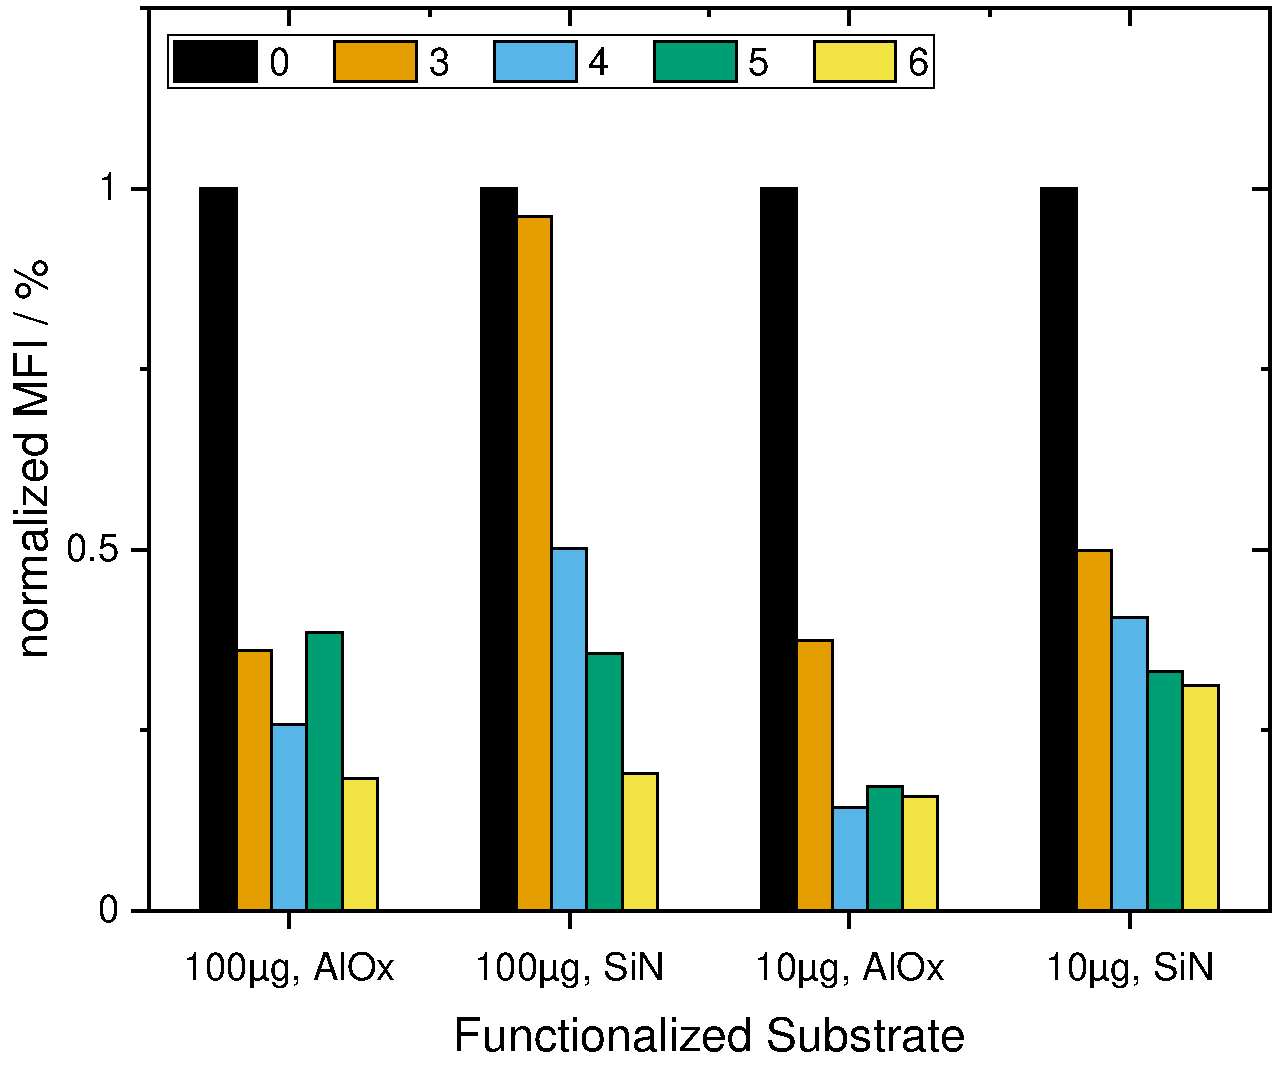
\includegraphics[height=150pt]{Ressources/ResultPlots/SurfaceFuncSiNAlOx}
	\capption{Surface Adsorption Stability of Neutravidin on \Gls{sin} and \Gls{alox}}{Blank with PBS and Blank substrate, corrected, then normalized, absolute protein per \textasciitilde \SI{25}{\milli\meter\square}}
	\label{fig:unsp:wash}
\end{figure}


\subsection{Covalent Attachment}
%\clearpage


\begin{figure}
	\centering
	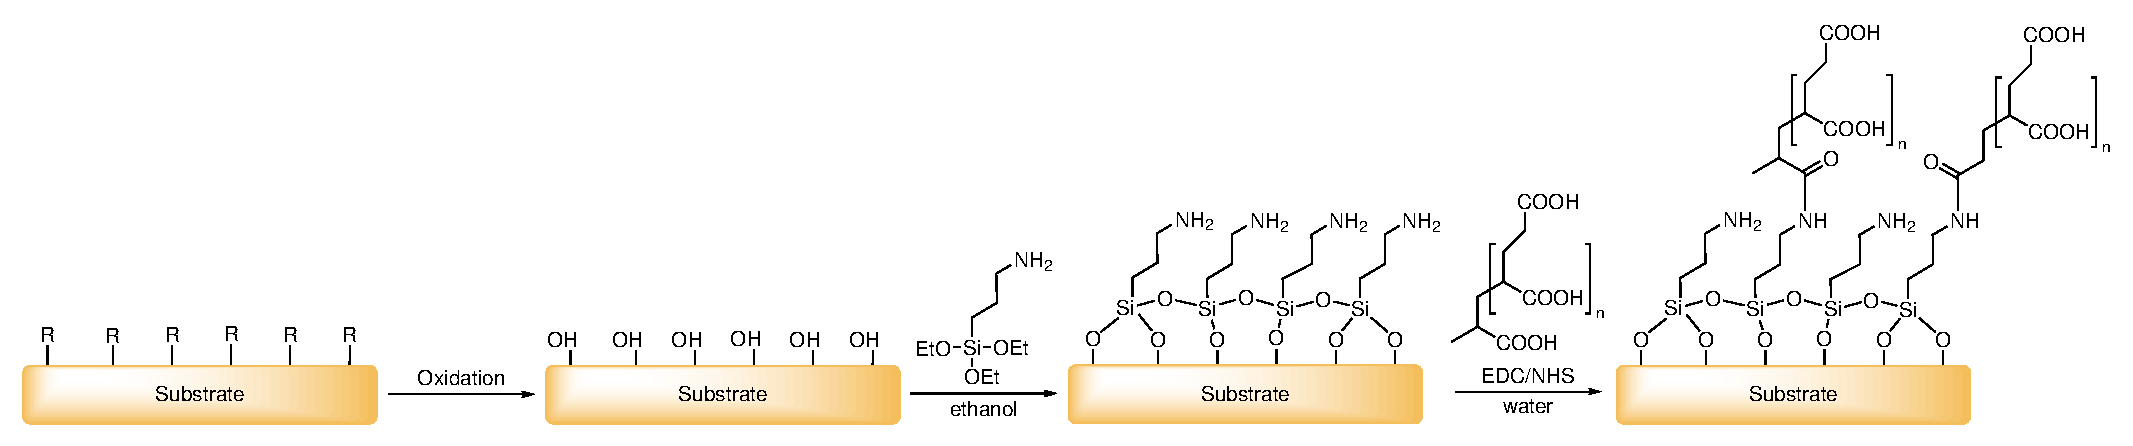
\includegraphics[width=1\linewidth]{Ressources/Chemistry/Substrate}
	\capption{General process chain of chemical surface modification}{Any substrate with various surface groups R (\textbf{a}) is oxidized to exhibit \gls{hydroxyl} groups.(\textbf{b}). Then a silane \gls{sam} is attached (\textbf{c}) and subsequently modified by carbodiimide chemistry with \gls{paa}. (\textbf{d})}
	\label{fig:chem:func:withPAA}
\end{figure}


\begin{figure}
	\centering
	\subfloat{
		\subfigimg[height=150pt]{a}{Ressources/Covalent/SerpentinesDensityCount}	
	} \hfill
	\subfloat{
		\subfigimg[height=150pt]{b}{Ressources/Covalent/NeutravidinTitration}	
	}
	\capption{Neutravidin Titration Fluorescence and Bead Capture Assay}{Relate count to area, then change MFI to counts \si{\per\micro\liter\per\milli\meter\squared}(\textbf{a}) Serpentine (\textbf{b}) Glass}
	\label{fig:coval:fluo}
\end{figure}

\subsubsection{Plasma-Based Approach}
\begin{figure}
	\centering
	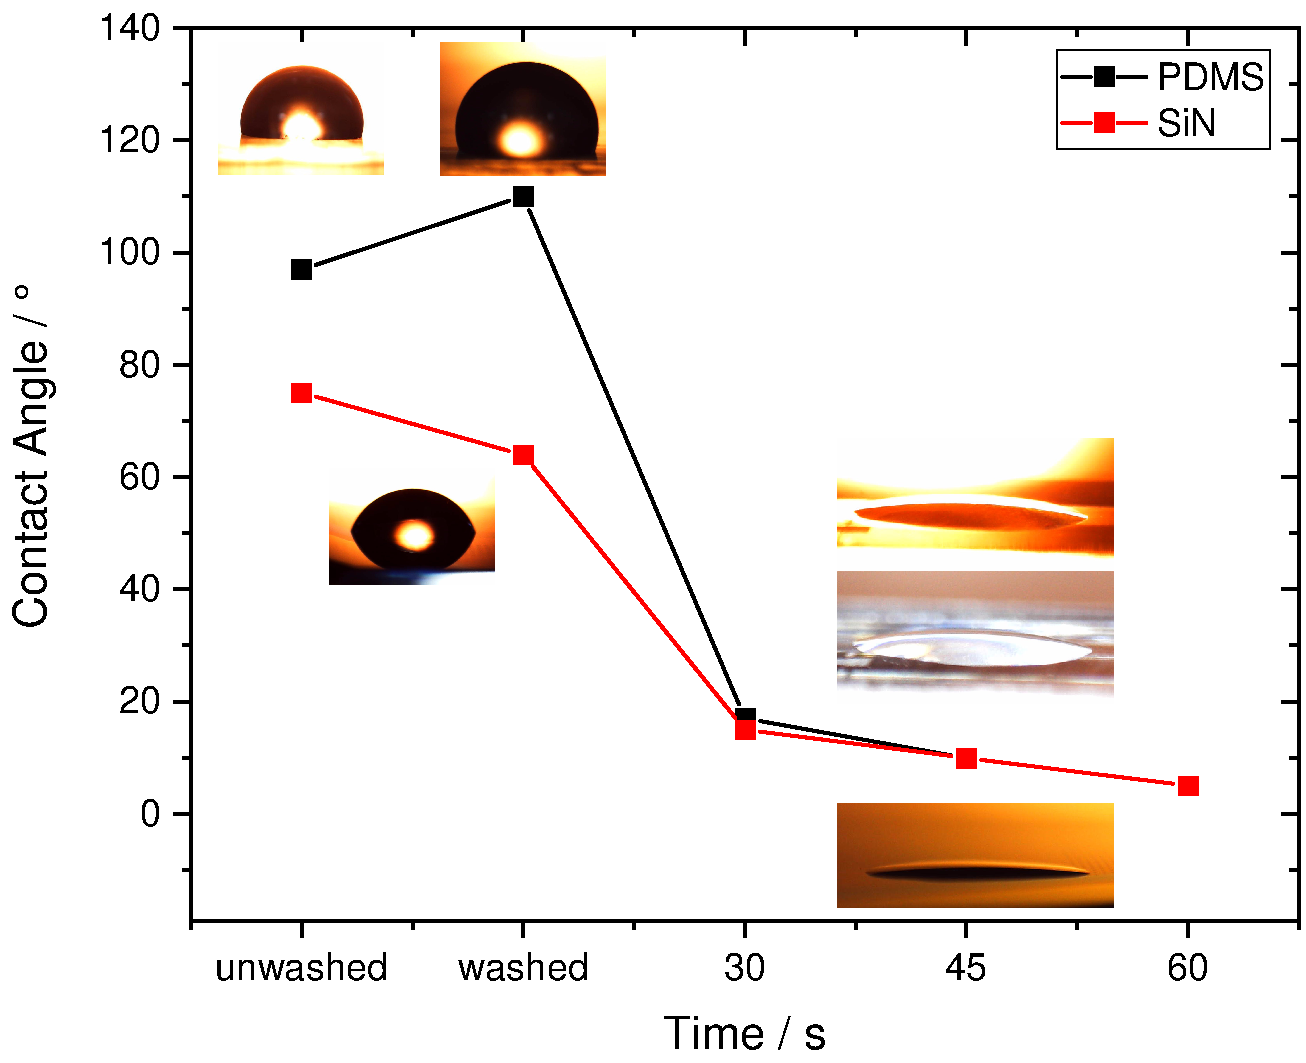
\includegraphics[height=150pt]{Ressources/ResultPlots/PDMS-sessileDrop}
	\capption{Hydrophbicity Analysis of \gls{pdms} under Plasma Exposure}{test123}
	\label{fig:coval:plasma}
\end{figure}


\subsubsection{Water-Based Approach}
Sonicate in Acetone and Water 5'
1:1 \gls{hcl}:Methanol
\gls{h2so4}
Treat for 30 min in light boiling water